\begin{center}
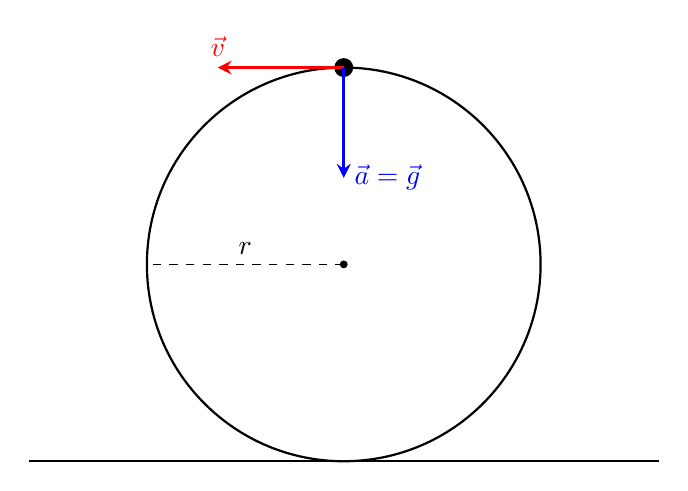
\begin{tikzpicture}[>=stealth]
 \draw[thick] (0,2.5) circle (2.5);
 \draw[thick] (-4,0) -- (4,0);
 \fill (0,2.5) circle (0.05);
 \draw[dashed] (0,2.5) -- (-2.5,2.5) node[midway, above] {$r$};
 \fill (0,5) circle (0.12);
 \draw[->, very thick, red] (0,5) -- (-1.6,5) node[above] {$\vec v$};
 \draw[->, very thick, blue] (0,5) -- (0,3.6) node[right] {$\vec a = \vec g$};
\end{tikzpicture}
\end{center}

\begin{abcliste}
\abc Im höchsten Punkt ist die Radialbeschleunigung $v^2/r$ nach unten gerichtet. Sie muss mindestens gleich $g$ sein, $v^2/r \geq g$:
\begin{align}
 v &= \vlF \\
   &= \sqrt{\gE\cdot\rl} \\
   &= \vl \approx \result{\vlP{0}{2}}
\end{align}

\abc Fährt die Bahn mit dieser Geschwindigkeit gleichförmig durch den ganzen Looping, so dauert die Fahrt
\begin{align}
 t &= \tlF \\
   &= \frac{2\pi\cdot\rl}{\vl} \\
   &= \tl \approx \result{\tlP{0}{2}}
\end{align}
In Wirklichkeit ist die Bahn unten schneller als oben; die Fahrt dauert deshalb etwas weniger lang.
\end{abcliste}
